\documentclass[11pt,spanish]{article}
\usepackage[utf8]{inputenc}
\usepackage{babel}
\usepackage{fullpage}
\usepackage{listings}
\usepackage{mathpazo}
\usepackage{enumitem}
\usepackage{courier}
\usepackage{xcolor}
\usepackage{textcomp}
\usepackage{amsmath}
\usepackage{amssymb}
\usepackage{tikz}
\usepackage{fancyhdr}
\usepackage{graphics}

\hyphenation{usua-rio usua-rios}

\newcommand{\titulo}{Certamen 2, sábado 14 de mayo de 2011}
\newcommand{\cc}[1]{\hfil\texttt{#1}\hfil}
\newcommand{\pond}[1]{[{\small\textbf{#1\%}}]}

\pagestyle{fancy}
\lhead{%
  {\Large\bfseries Programación---\titulo} \\
  Nombre: \nombre\hfill
  Rol:    \rol
  \vspace{2ex}
}
\chead{}\rhead{}\lfoot{}\cfoot{}\rfoot{}
\renewcommand{\headrulewidth}{0pt}
\addtolength{\headheight}{7ex}
\headsep=4ex


\newcommand{\onelinerule}{\rule[2.3ex]{0pt}{0pt}}
\newcommand{\twolinerule}{\rule[6.2ex]{0pt}{0pt}}
\newcommand{\respuesta}{\framebox[\textwidth]{\twolinerule}}
\newcommand{\nombre}{%
  \begin{tikzpicture}[xscale=.4,yscale=.7]
    \draw (0, 0) rectangle (22, 1);
  \end{tikzpicture}%
}
%\newcommand{\rol}   {\framebox[0.3\textwidth]{\onelinerule}}
\newcommand{\rol}{%
  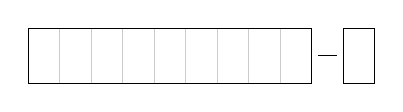
\begin{tikzpicture}[xscale=.4,yscale=.7]
    \draw[gray!40] ( 0, 0) grid      ( 9, 1);
    \draw          ( 0, 0) rectangle ( 9, 1);
    \draw          (10, 0) rectangle (11, 1);
    \draw (9 + .2, .5) -- (10 - .2, .5);
  \end{tikzpicture}%
}
\newcommand{\li}{\lstinline}
\providecommand{\pond}[1]{[{\small\textbf{#1\%}}]}

\lstdefinelanguage{py}{%
  classoffset=0,%
    morekeywords={%
      False,class,finally,is,return,None,continue,for,lambda,try,%
      True,def,from,nonlocal,while,and,del,global,not,with,print,%
      as,elif,if,or,yield,assert,else,import,pass,break,except,in,raise},%
    keywordstyle=\color{black!80}\bfseries,%
  classoffset=1,
    morekeywords={int,float,str,abs,len,raw_input,exit,range,min,max,%
      set,dict,tuple,list,bool,complex,round,sum,all,any,zip,map,filter,%
      sorted,reversed,dir,file,frozenset,open,%
      array,zeros,ones,arange,linspace,eye,diag,dot},
    keywordstyle=\color{black!50}\bfseries,%
  classoffset=0,%
  sensitive=true,%
  morecomment=[l]\#,%
  morestring=[b]',%
  morestring=[b]",%
  stringstyle=\em,%
}

\lstdefinelanguage{testcase}{%
  moredelim=[is][\bfseries]{`}{`},%
  backgroundcolor=\color{gray!20},%
}

\lstdefinelanguage{file}{%
  frame=single,%
}

\lstset{language=py}
\lstset{basicstyle=\ttfamily}
\lstset{columns=fixed}
\lstset{upquote=true}
\lstset{showstringspaces=false}
\lstset{rangeprefix=\#\ }
\lstset{includerangemarker=false}

\newlist{certamen}{enumerate}{1}
\setlist[certamen]{%
  label=\arabic*.,
  font=\LARGE\bfseries,%
  labelindent=-.5in,%
  leftmargin=0pt,%
  labelsep=1em%
}



\begin{document}

  \begin{enumerate}[font=\Large\bfseries]

    \item
      \pond{25}
      Indique qué es lo que imprimen los siguientes programas.

      \foreach \x in {1,2,...,8} {
        \noindent
        \begin{minipage}[b]{19.8em}
          \lstinputlisting{p\x.py}
          \framebox[18em]{\rule[6ex]{0pt}{0pt}}
          \vspace{0.7em}
        \end{minipage}
      }

    \newpage
    \item
      \pond{25}
      \begin{minipage}[t]{.50\textwidth}
  \parskip=1ex
  El \emph{rango} de un conjunto de datos reales
  es la dife\-rencia entre el mayor y el menor de los datos.

  Escriba un programa que le pregunte al usuario
  cuántos datos serán ingresados,
  le pida ingresar los datos uno por uno
  y finalmente entregue como resultado
  el rango de los datos.
\end{minipage}
\hfill
\begin{minipage}[t]{.43\textwidth}
  \lstinputlisting[language=testcase,frame=single]{rango/caso3.txt}
\end{minipage}



    \newpage
    \item
      \pond{25}
      La banda de rock Strip'n Split
ha concluído su gira mundial.
La información de cada uno de sus conciertos
está almacenada en una lista
en orden cronológico.

\begin{minipage}[t]{.45\textwidth}
  Cada elemento de la lista
  es un diccionario con tres llaves:
  \li!'ciudad'!, \li!'publico'! y \li!'canciones'!.
  El valor asociado a \li!'publico'!
  es la cantidad de personas que asistió al concierto,
  y el asociado a \li!'canciones'!
  es la lista de las canciones que fueron tocadas
  en ese concierto.

  \begin{enumerate}
    \item
      Escriba una función llamada
      \li!cuantos_escucharon(c)!,
      que retorne la cantidad de personas
      que escucharon la canción \li!c!.
    \item
      Escriba una función llamada
      \li!mismo_concierto(c1, c2)!,
      que retorne \li!True! o \li!False!
      para indicar si las canciones \li!c1! y \li!c2!
      fueron tocadas alguna vez en el mismo concierto.
  \end{enumerate}
\end{minipage}
\hspace{2em}
\begin{minipage}[t]{.55\textwidth}
  \small
  \lstinputlisting[linerange=CONCIERTOS-FIN\ CONCIERTOS]
     {strip-n-split/pauta3-4.py}
\end{minipage}



    \newpage
    \item
      \pond{25}
      (Este ejercicio es una continuación del anterior).

Para guardar la información sobre cuáles de sus usuarios son amigos entre sí,
Fookbace utiliza el conjunto \li!amistades!,
que contiene tuplas con los códigos de dos usuarios.
Si la tupla \li!(a, b)! está dentro del conjunto,
significa que los usuarios con códigos \li!a! y \li!b! son amigos.
En todas las tuplas se cumple que \(\text{\li!a!} < \text{\li!b!}\).
\lstinputlisting[linerange=AMIGOS-FIN\ AMIGOS]{fookbace/pauta3-4.py}
\begin{enumerate}
  \item Escriba la función \li!obtener_amigos(u)!,
    que retorne el conjunto de los códigos
    de los amigos de \li!u!.
  \item Escriba la función \li!recomendar_amigos(u)!,
    que retorne el conjunto de los códigos
    de los usuarios que cumplen todas estas condiciones a la vez:
    \begin{itemize}
      \item son amigos de un amigo de \li!u!,
      \item no son amigos de \li!u!,
      \item viven en la misma ciudad que \li!u!, y
      \item tienen menos de diez años de diferencia con \li!u!.
    \end{itemize}
\end{enumerate}
En ambas funciones,
el parámetro \li!u! es el código de un usuario,
y el valor de retorno es un conjunto de códigos de usuarios.
Recuerde que \li!c.add(x)! agrega el valor \li!x! al conjunto \li!c!.



  \end{enumerate}
\end{document}

